
\documentclass[11pt,a4paper]{article}

% ============================================================
% DTU BIOENGINEERING 27020 - NEURO GROUP 8
% SUPPLEMENTARY QUANTITATIVE ANALYSIS
%
% All model performance and cost values are hypothetical.
% Compile with pdfLaTeX on Overleaf.
% ============================================================

% ---------------------- PACKAGES ----------------------------
\usepackage[T1]{fontenc}
\usepackage[utf8]{inputenc}
\usepackage{lmodern}
\usepackage[english]{babel}
\usepackage[a4paper,margin=20mm]{geometry}
\usepackage{amsmath,amssymb}
\usepackage{booktabs,tabularx,array}
\usepackage{graphicx}
\usepackage{xcolor}
\usepackage{microtype}
\usepackage{tikz}
\usetikzlibrary{arrows.meta,positioning}
\usepackage{pgfplots}
\pgfplotsset{compat=1.18}
\usepackage{hyperref}
\usepackage{fancyhdr}
\usepackage{enumitem}
\usepackage{float}

% ---------------------- STYLING -----------------------------
\definecolor{DTUblue}{HTML}{103455}
\definecolor{DTUaccent}{HTML}{297BA4}
\definecolor{DTUlight}{HTML}{EDF5F9}
\definecolor{DTUgreen}{HTML}{287F68}
\definecolor{DTUred}{HTML}{BA514B}

\hypersetup{
    colorlinks=true,
    linkcolor=DTUblue,
    urlcolor=DTUaccent
}

\pagestyle{fancy}
\fancyhf{}
\lhead{\small\color{DTUblue}NEURO 8 -- Quantitative Analysis}
\rhead{\small\thepage}
\renewcommand{\headrulewidth}{0.4pt}
\setlength{\headheight}{14pt}

\setlength{\parindent}{0pt}
\setlength{\parskip}{5pt}
\renewcommand{\arraystretch}{1.18}
\setlist[itemize]{nosep,leftmargin=*}

\newcommand{\subheading}[1]{%
    \vspace{3mm}
    {\large\bfseries\color{DTUblue}#1}\par
}

% ============================================================
\begin{document}
% ============================================================

{\LARGE\bfseries\color{DTUblue}
Supplementary Quantitative Analysis\par}

\vspace{2mm}

{\large
Early \& Personalized Alzheimer's Prediction\par}

\vspace{2mm}

\textbf{DTU Bioengineering 27020 -- NEURO Group 8}

\vspace{4mm}

\noindent\fcolorbox{DTUblue}{DTUlight}{%
\begin{minipage}{0.94\linewidth}
\textbf{Purpose.}
Evaluate the potential clinical and economic feasibility
of a proposed blood-first Alzheimer's risk assessment
pathway, guided by a multimodal teacher model.

\medskip

\textbf{Important:}
All model-performance figures, costs and cohort assumptions
in this document are hypothetical.
Neither the teacher nor student model has been trained
or clinically validated as part of this project.
\end{minipage}
}

% ============================================================
\section{Proposed Clinical Pathway}
% ============================================================

The proposed research framework uses two models:

\begin{itemize}
    \item \textbf{Multimodal teacher:}
    Integrates longitudinal MRI, PET, EEG and blood-based
    measurements to estimate future Alzheimer's risk.

    \item \textbf{Blood-only student:}
    Uses accessible blood biomarkers, including
    A$\beta$42/40 and p-tau217, with training guidance
    from the multimodal teacher.
\end{itemize}

For this numerical scenario, the student is assumed
to estimate the probability of developing clinically
diagnosed Alzheimer's dementia within five years.

Patients with positive blood-screening results are
referred for additional MRI assessment. In practice,
MRI alone would not establish an Alzheimer's diagnosis;
clinical evaluation and other diagnostic tests may
also be necessary.

The teacher model is a proposed research and training
component, not a test that every patient must receive.

% ============================================================
\section{Assumptions}
% ============================================================

\begin{table}[H]
\centering
\caption{Hypothetical baseline parameters.}
\begin{tabularx}{\linewidth}{@{}Xrl@{}}
\toprule
\textbf{Parameter} & \textbf{Value} & \textbf{Symbol} \\
\midrule
Patients screened & 10,000 & $N$ \\
Five-year disease risk in cohort & 10\% & $p$ \\
Student sensitivity & 85\% & $Se$ \\
Student specificity & 90\% & $Sp$ \\
Blood biomarker test cost & 500 DKK & $C_b$ \\
MRI examination cost & 5,000 DKK & $C_m$ \\
\bottomrule
\end{tabularx}
\end{table}

The assumed disease risk refers to a selected,
at-risk clinical cohort. It is \textbf{not} an estimate
of Alzheimer's incidence in the general population.

The assumed costs are illustrative unit prices,
not verified Danish healthcare tariffs.
All patients are assumed to complete the blood test,
and all positive screens are assumed to receive MRI.

% ============================================================
\section{Predictive Performance}
% ============================================================

\subheading{Confusion Matrix}

The number of patients who develop the defined outcome
within five years is:

\[
N_D=Np=10\,000(0.10)=1\,000.
\]

The remaining 9,000 patients do not develop
the defined outcome during that interval.

Using the assumed sensitivity and specificity:

\begin{align*}
TP &= NpSe = 850,\\
FN &= Np(1-Se) = 150,\\
FP &= N(1-p)(1-Sp) = 900,\\
TN &= N(1-p)Sp = 8\,100.
\end{align*}

\begin{table}[H]
\centering
\caption{Hypothetical blood-only screening results.}
\begin{tabular}{@{}lrrr@{}}
\toprule
& \textbf{Future case}
& \textbf{Non-case}
& \textbf{Total} \\
\midrule
Positive screen & 850 & 900 & 1,750 \\
Negative screen & 150 & 8,100 & 8,250 \\
\midrule
Total & 1,000 & 9,000 & 10,000 \\
\bottomrule
\end{tabular}
\end{table}

\subheading{Clinical Performance Measures}

Positive predictive value:

\[
PPV=\frac{TP}{TP+FP}
=\frac{850}{1750}
=\boxed{48.6\%}.
\]

Negative predictive value:

\[
NPV=\frac{TN}{TN+FN}
=\frac{8100}{8250}
=\boxed{98.2\%}.
\]

Proportion referred for MRI:

\[
f=\frac{TP+FP}{N}
=\frac{1750}{10000}
=\boxed{17.5\%}.
\]

\textbf{Interpretation:}
The pathway flags 850 of the 1,000 future cases
but misses 150. Of the 1,750 positive screens,
900 are false positives with respect to the
defined five-year outcome.

% ============================================================
\subheading{Screening Pathway}
% ============================================================

\begin{figure}[H]
\centering
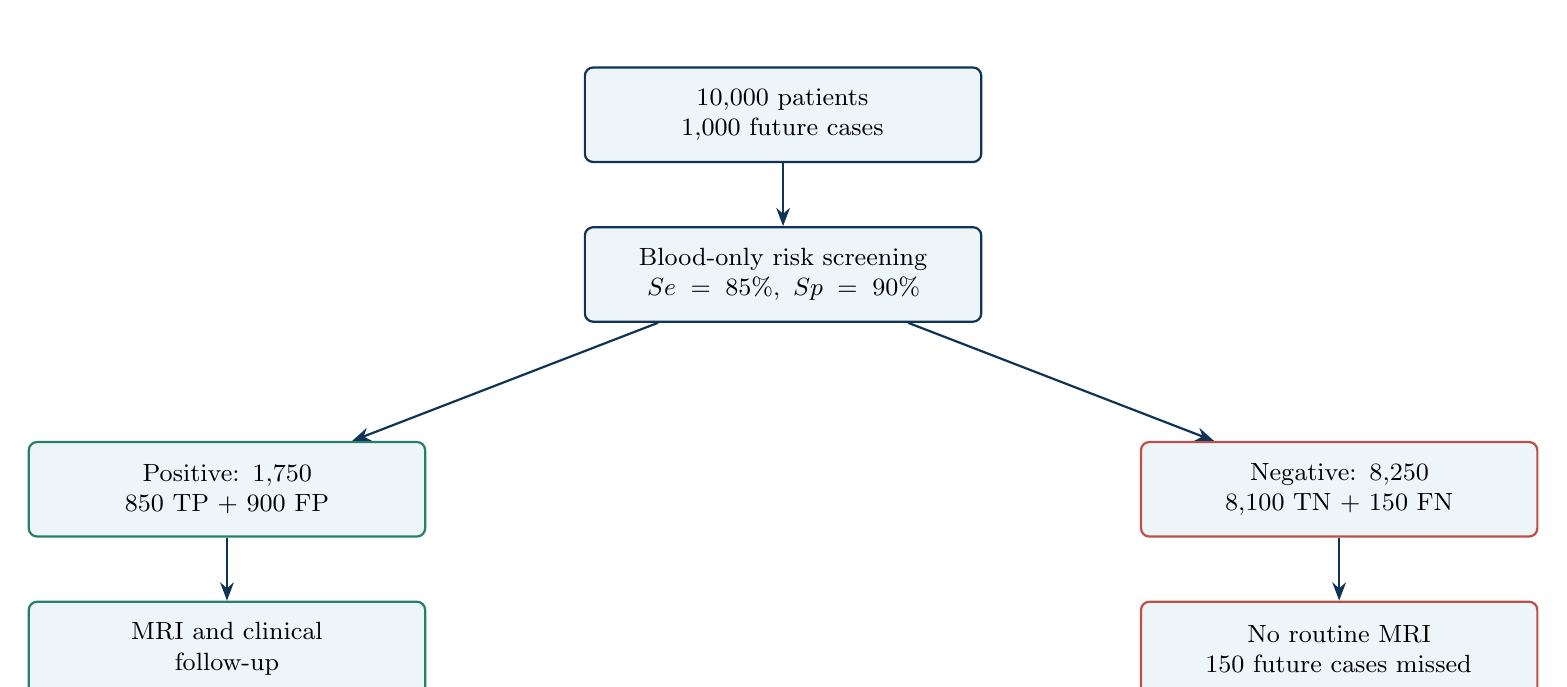
\begin{tikzpicture}[
    >=Stealth,
    font=\small,
    block/.style={
        draw=DTUblue,
        thick,
        rounded corners=3pt,
        fill=DTUlight,
        align=center,
        text width=48mm,
        minimum height=12mm
    },
    positive/.style={
        block,
        draw=DTUgreen
    },
    negative/.style={
        block,
        draw=DTUred
    },
    arrow/.style={->,thick,draw=DTUblue}
]

\node[block] (cohort)
    {10,000 patients\\
     1,000 future cases};

\node[block,below=8mm of cohort] (test)
    {Blood-only risk screening\\
     $Se=85\%,\ Sp=90\%$};

\node[positive,
      below left=15mm and 20mm of test] (pos)
    {Positive: 1,750\\
     850 TP + 900 FP};

\node[negative,
      below right=15mm and 20mm of test] (neg)
    {Negative: 8,250\\
     8,100 TN + 150 FN};

\node[positive,below=8mm of pos] (mri)
    {MRI and clinical\\
     follow-up};

\node[negative,below=8mm of neg] (miss)
    {No routine MRI\\
     150 future cases missed};

\draw[arrow] (cohort) -- (test);
\draw[arrow] (test) -- (pos);
\draw[arrow] (test) -- (neg);
\draw[arrow] (pos) -- (mri);
\draw[arrow] (neg) -- (miss);

\end{tikzpicture}

\caption{
Illustrative screening and referral pathway.
The false-negative group highlights the clinical
risk of relying on blood-first screening.
}
\end{figure}

% ============================================================
\section{Economic Feasibility}
% ============================================================

We compare two simplified examination strategies:

\begin{itemize}
    \item \textbf{Universal testing:}
    All patients receive a blood test and MRI.

    \item \textbf{Blood-first testing:}
    All patients receive a blood test, followed
    by MRI only after a positive screen.
\end{itemize}

This is a comparison of examination pathways,
\textbf{not} the total cost of operating the
full MRI--PET--EEG--blood teacher model.

\subheading{Universal Testing}

\[
C_{\mathrm{universal}}
=N(C_b+C_m).
\]

\[
=10\,000(500+5000)
=\boxed{55\,000\,000\ \mathrm{DKK}}.
\]

\subheading{Blood-First Testing}

\[
C_{\mathrm{blood-first}}
=NC_b+(TP+FP)C_m.
\]

\[
=10\,000(500)+1750(5000).
\]

\[
=\boxed{13\,750\,000\ \mathrm{DKK}}.
\]

\subheading{Estimated Cost Reduction}

\[
\Delta C
=55\,000\,000-13\,750\,000
=41\,250\,000\ \mathrm{DKK}.
\]

\[
S=\frac{\Delta C}{C_{\mathrm{universal}}}
\times100\%
=\boxed{75\%}.
\]

\begin{table}[H]
\centering
\caption{Direct examination-cost comparison.}
\begin{tabularx}{\linewidth}{@{}Xrr@{}}
\toprule
\textbf{Measure}
& \textbf{Universal}
& \textbf{Blood-first} \\
\midrule
Blood tests & 10,000 & 10,000 \\
MRI examinations & 10,000 & 1,750 \\
Total cost (M DKK) & 55.00 & 13.75 \\
Cost per patient (DKK) & 5,500 & 1,375 \\
\bottomrule
\end{tabularx}
\end{table}

\begin{figure}[H]
\centering
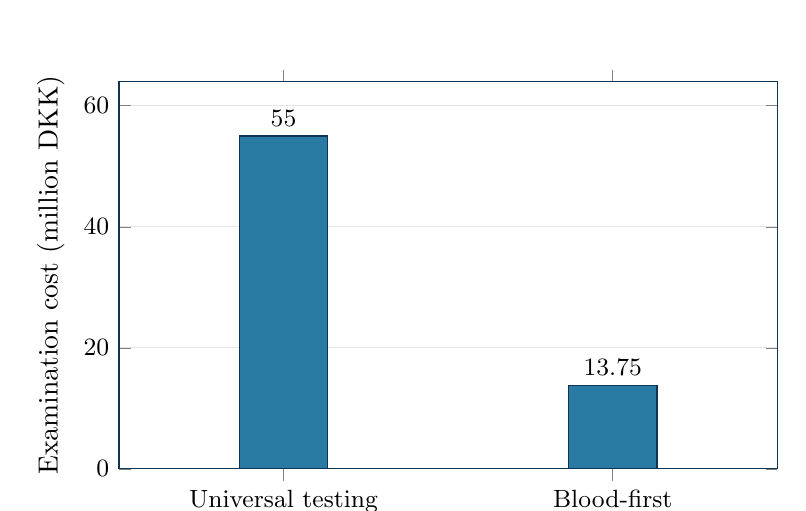
\begin{tikzpicture}
\begin{axis}[
    width=0.82\linewidth,
    height=65mm,
    ybar,
    bar width=32pt,
    xmin=0.5,
    xmax=2.5,
    ymin=0,
    ymax=64,
    xtick={1,2},
    xticklabels={Universal testing,Blood-first},
    ylabel={Examination cost (million DKK)},
    ymajorgrids=true,
    grid style={gray!20},
    nodes near coords,
    every node near coord/.append style={
        font=\small,
        color=black
    },
    tick label style={font=\small},
    axis line style={draw=DTUblue}
]
\addplot[
    draw=DTUblue,
    fill=DTUaccent
] coordinates {
    (1,55)
    (2,13.75)
};
\end{axis}
\end{tikzpicture}
\caption{
Hypothetical examination costs for 10,000 patients.
Model development, clinical follow-up and
other healthcare costs are excluded.
}
\end{figure}

\textbf{Interpretation:}
Under these assumptions, blood-first testing
reduces the number of MRI examinations by 82.5\%
and direct examination expenditure by 75\%.

The saving is conditional on the model's screening
accuracy and does not establish clinical safety
or overall cost-effectiveness.

% ============================================================
\section{Scalability}
% ============================================================

The general referral fraction is:

\[
f=pSe+(1-p)(1-Sp).
\]

Therefore, for cohort size $N$:

\[
C_{\mathrm{blood-first}}
=N\left(C_b+fC_m\right).
\]

If disease risk, model performance and unit prices
remain unchanged, the number of examinations
and direct examination costs scale linearly.

\begin{table}[H]
\centering
\caption{Hypothetical scaling with cohort size.}
\small
\begin{tabular}{@{}rrrrr@{}}
\toprule
\textbf{Patients} &
\textbf{MRI} &
\textbf{Missed} &
\textbf{Universal} &
\textbf{Blood-first} \\
& \textbf{referrals} &
\textbf{cases} &
\textbf{M DKK} &
\textbf{M DKK} \\
\midrule
1,000 & 175 & 15 & 5.50 & 1.375 \\
10,000 & 1,750 & 150 & 55.00 & 13.750 \\
100,000 & 17,500 & 1,500 & 550.00 & 137.500 \\
\bottomrule
\end{tabular}
\end{table}

Actual implementation may not scale linearly
because laboratory capacity, MRI availability,
staffing and infrastructure costs can change
as patient volume increases.

% ============================================================
\section{Sensitivity Analysis}
% ============================================================

The baseline economic result depends on
the model's sensitivity and specificity.

\subheading{Effect of Specificity}

Keeping sensitivity at 85\%:

\begin{table}[H]
\centering
\caption{Effect of specificity on costs and referrals.}
\begin{tabular}{@{}rrrrr@{}}
\toprule
\textbf{Sp} &
\textbf{FP} &
\textbf{MRI referrals} &
\textbf{Cost (M DKK)} &
\textbf{Saving} \\
\midrule
85\% & 1,350 & 2,200 & 16.00 & 70.9\% \\
90\% & 900 & 1,750 & 13.75 & 75.0\% \\
95\% & 450 & 1,300 & 11.50 & 79.1\% \\
\bottomrule
\end{tabular}
\end{table}

Higher specificity reduces unnecessary
MRI referrals, while the assumed number
of missed future cases remains 150.

\subheading{Effect of Sensitivity}

Keeping specificity at 90\%:

\begin{table}[H]
\centering
\caption{Effect of sensitivity on missed cases.}
\begin{tabular}{@{}rrrrr@{}}
\toprule
\textbf{Se} &
\textbf{TP} &
\textbf{FN} &
\textbf{MRI referrals} &
\textbf{Cost (M DKK)} \\
\midrule
75\% & 750 & 250 & 1,650 & 13.25 \\
85\% & 850 & 150 & 1,750 & 13.75 \\
95\% & 950 & 50 & 1,850 & 14.25 \\
\bottomrule
\end{tabular}
\end{table}

Higher sensitivity reduces missed cases,
but increases MRI referrals in this model.

\subheading{Cost Versus MRI Referral Rate}

For a general referral rate $f$:

\[
C_{\mathrm{patient}}=C_b+fC_m.
\]

\begin{figure}[H]
\centering
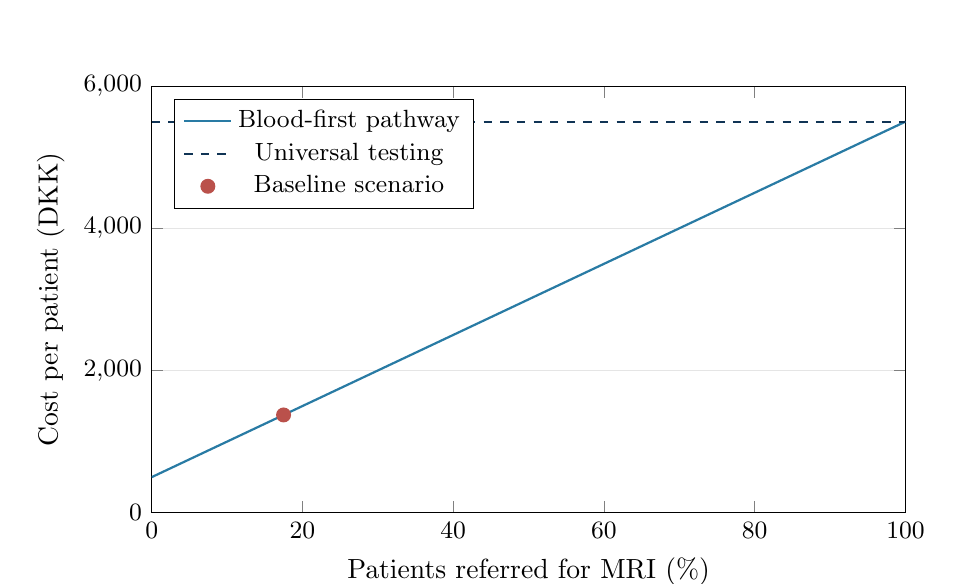
\begin{tikzpicture}
\begin{axis}[
    width=0.92\linewidth,
    height=70mm,
    xmin=0,
    xmax=100,
    ymin=0,
    ymax=6000,
    xlabel={Patients referred for MRI (\%)},
    ylabel={Cost per patient (DKK)},
    xtick={0,20,40,60,80,100},
    ymajorgrids=true,
    grid style={gray!20},
    legend pos=north west,
    legend style={font=\small},
    tick label style={font=\small}
]

\addplot[
    thick,
    color=DTUaccent,
    mark=none
] coordinates {
    (0,500)
    (17.5,1375)
    (25,1750)
    (50,3000)
    (75,4250)
    (100,5500)
};
\addlegendentry{Blood-first pathway}

\addplot[
    thick,
    dashed,
    color=DTUblue,
    mark=none
] coordinates {
    (0,5500)
    (100,5500)
};
\addlegendentry{Universal testing}

\addplot[
    only marks,
    mark=*,
    mark size=2.5pt,
    color=DTUred
] coordinates {
    (17.5,1375)
};
\addlegendentry{Baseline scenario}

\end{axis}
\end{tikzpicture}

\caption{
Examination expenditure per patient as a function
of the proportion referred for MRI.
The baseline scenario refers 17.5\% of patients.
}
\end{figure}

% ============================================================
\section{Multimodal Teacher Versus Blood-Only Student}
% ============================================================

The project's central research question asks
how much predictive performance could be retained
after removing imaging and EEG inputs.

Both models would need to be evaluated on
the same independent patient cohort,
with the same clinical endpoint and
five-year prediction horizon.

The following comparison is hypothetical.

\begin{table}[H]
\centering
\caption{Illustrative teacher--student comparison.}
\begin{tabularx}{\linewidth}{@{}Xcc@{}}
\toprule
\textbf{Metric} &
\textbf{Teacher} &
\textbf{Student} \\
\midrule
Input data & Multimodal & Blood only \\
AUROC & 0.93 & 0.87 \\
Sensitivity & 90\% & 85\% \\
Specificity & 93\% & 90\% \\
False negatives per 1,000 future cases
& 100 & 150 \\
\bottomrule
\end{tabularx}
\end{table}

The hypothetical AUROC difference is:

\[
\Delta\mathrm{AUROC}
=0.93-0.87
=\boxed{0.06}.
\]

This illustrates one way to quantify
the performance trade-off.

However, it does not establish how much
biological information is retained.
AUROC also does not assess probability calibration.

A real evaluation should include:

\begin{itemize}
    \item AUROC and area under the
    precision--recall curve (AUPRC).
    \item Sensitivity, specificity, PPV and NPV.
    \item Probability calibration and Brier score.
    \item Performance across populations
    and clinically relevant subgroups.
    \item External validation with longitudinal
    clinical follow-up.
\end{itemize}

\textbf{No teacher--student performance comparison
has been experimentally established in this project.}

% ============================================================
\section{Limitations and Clinical Feasibility}
% ============================================================

\begin{enumerate}[leftmargin=*]
    \item \textbf{Hypothetical performance:}
    Sensitivity, specificity and AUROC values
    are assumptions, not observed results.

    \item \textbf{Assumed pricing:}
    Unit costs are illustrative and exclude
    model development, maintenance,
    staff time and infrastructure.

    \item \textbf{Follow-up costs:}
    MRI may not be sufficient for clinical
    diagnosis, and additional testing
    or specialist assessment may be needed.

    \item \textbf{False negatives:}
    In the baseline scenario, 150 future cases
    are missed by blood screening.
    Clinical reassessment may still be necessary.

    \item \textbf{Dataset limitations:}
    Longitudinal MRI, PET, EEG and blood data
    must be aligned across patients and time.
    Selection bias, missing data and leakage
    must be addressed.

    \item \textbf{Deployment:}
    Clinical usefulness requires external
    validation, regulatory assessment,
    patient privacy safeguards and
    demonstration of an acceptable
    benefit--harm balance.
\end{enumerate}

% ============================================================
\section{Conclusion}
% ============================================================

The proposed teacher--student system is
technically plausible as a research concept,
but its predictive and economic benefits
remain unverified.

Under the hypothetical assumptions used here,
a blood-first screening pathway reduces
direct examination costs by 75\% relative to
blood testing and MRI for every patient.

However, this pathway would miss 150 of the
1,000 patients developing the defined
five-year clinical outcome.

\noindent\fcolorbox{DTUblue}{DTUlight}{%
\begin{minipage}{0.94\linewidth}
\textbf{Key takeaway}

\medskip

\textbf{10,000 patients}
$\;\longrightarrow\;$
\textbf{1,750 MRI referrals}

\textbf{55M DKK}
$\;\longrightarrow\;$
\textbf{13.75M DKK}

\textbf{75\% lower examination costs},
but \textbf{150 missed future cases}.

\medskip

\textit{
These are illustrative scenario results,
not validated model predictions or
demonstrated healthcare savings.
}
\end{minipage}
}

\vspace{4mm}

The next research step is to train and compare
teacher and student models using real longitudinal
data, then evaluate whether the reduction in
examination burden justifies the potential
loss in predictive performance.

% ============================================================
\section*{Background Literature}
% ============================================================

The following sources provide biological
and clinical context, but do not substantiate
the hypothetical numerical assumptions above.

\begin{itemize}
    \item World Health Organization.
    \textit{Dementia} (2026).
    \url{https://www.who.int/news-room/fact-sheets/detail/dementia}

    \item Fu, W. and Ho, P. C.-L.
    \textit{Blood-based biomarkers for Alzheimer's
    disease: Advances in early detection and
    monitoring of age-related neurodegeneration}.
    Ageing Research Reviews (2026).
    \href{https://doi.org/10.1016/j.arr.2026.103058}
    {DOI: 10.1016/j.arr.2026.103058}

    \item Therriault, J. et al.
    \textit{Blood phosphorylated tau for
    the diagnosis of Alzheimer's disease:
    a systematic review and meta-analysis}.
    The Lancet Neurology (2025).
    \href{https://doi.org/10.1016/S1474-4422(25)00227-3}
    {DOI: 10.1016/S1474-4422(25)00227-3}
\end{itemize}

\end{document}
